\begin{figure*}[h]
\providecommand{\width}{}
\renewcommand{\width}{0.62\textwidth}
\centering
\begin{subfigure}[t]{\width}
\rot{\hspace{4.6em}\method}
\hspace{.5em}
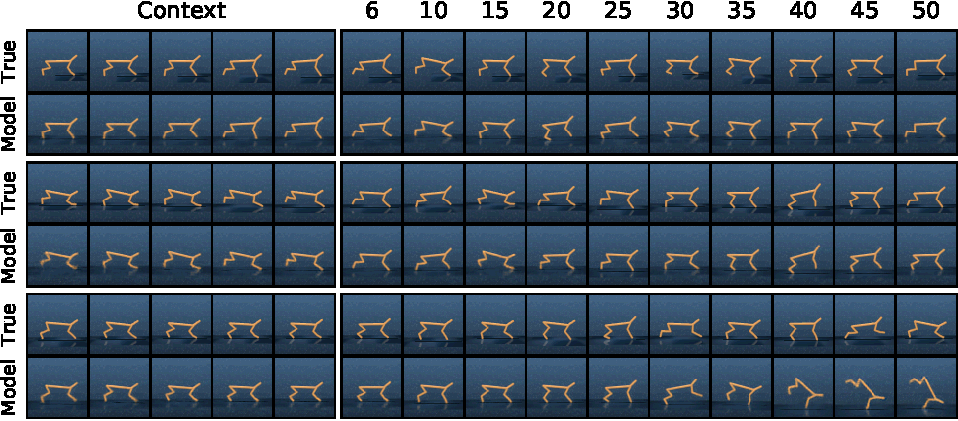
\includegraphics[width=\textwidth]{prediction/cheetah-planet}
\end{subfigure} \\
\vspace{2ex}
\begin{subfigure}[t]{\width}
\rot{\hspace{1.3em}\method + Overshooting}
\hspace{.5em}
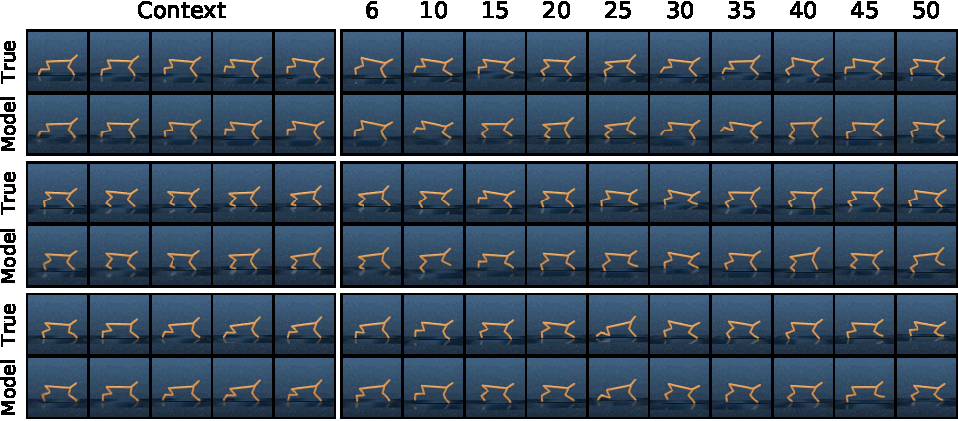
\includegraphics[width=\textwidth]{prediction/cheetah-latov}
\end{subfigure} \\
\vspace{2ex}
\begin{subfigure}[t]{\width}
\rot{\hspace{1.8em}Deterministic (GRU)}
\hspace{.5em}
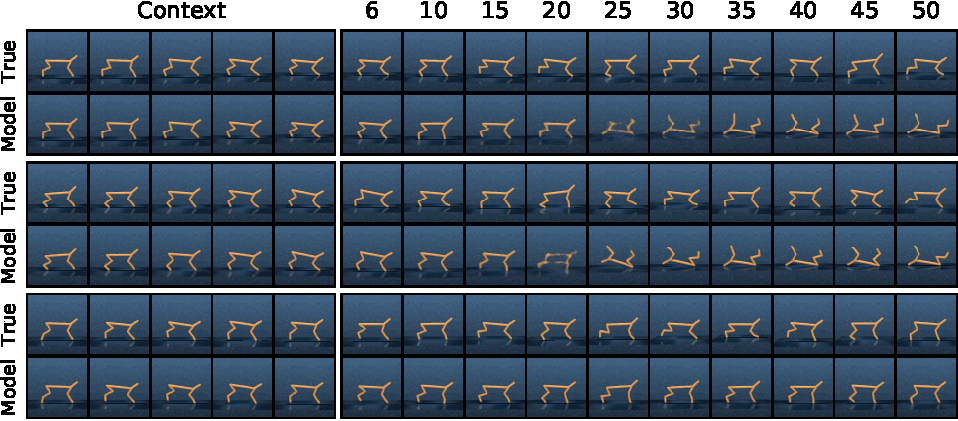
\includegraphics[width=\textwidth]{prediction/cheetah-rnn}
\end{subfigure} \\
\vspace{2ex}
\begin{subfigure}[t]{\width}
\rot{\hspace{2.5em}Stochastic (SSM)}
\hspace{.5em}
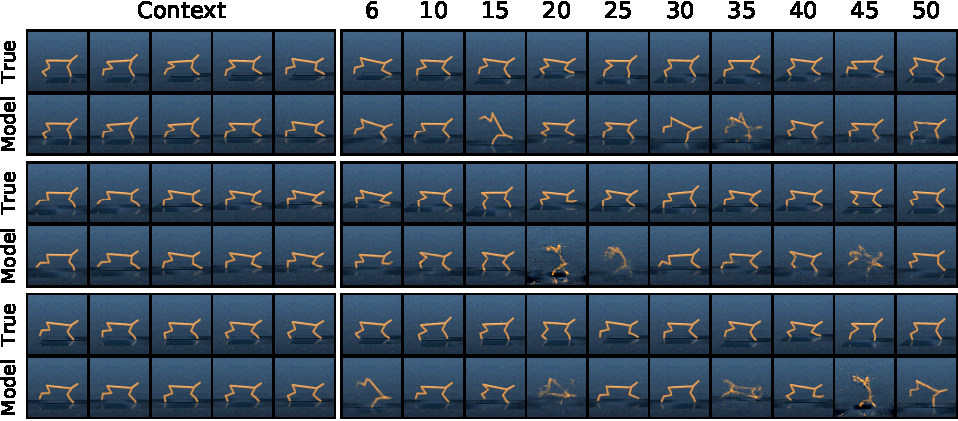
\includegraphics[width=\textwidth]{prediction/cheetah-ssm}
\end{subfigure} \\
\caption{Open-loop video predictions for test episodes. The \mbox{columns 1--5} show reconstructed context frames and the remaining images are generated open-loop. Our RSSM achieves pixel-accurate predictions for 50 steps into the future in the cheetah environment. We randomly selected action sequences from test episodes collected with action noise alongside the training episodes.}
\label{fig:prediction}
\vspace{-0.2in}
\end{figure*}